\documentclass[paper=8.27in:11.69in, DIV=calc]{scrartcl}
\usepackage{geometry}
\usepackage{graphics,graphicx}
\usepackage{pdfpages}
\usepackage{hyperref}
\usepackage{enumitem}
\usepackage{amsmath}
\usepackage{minibox}
\newcounter{numbers}
\newcommand\printnumbers{\refstepcounter{numbers}\thenumbers}
\newcounter{answers}
\newcommand\printanswers{\refstepcounter{answers}\theanswers}

\begin{document}

\textbf{\begin{center}
\begin{Large}
CSCI 6339 Theoretical Foundations of Computer Science\\
Homework 1\\
Due is 09/20/2020 23:59\\
Ulvi Bajarani\\
Student ID 20539914\\
E-mail: ulvi.bajarani01@utrgv.edu\\
\end{Large}
\end{center}}

\newpage
\noindent \begin{center}
\textbf{Questions and Answers:}
\end{center}


\textbf{Problem \printnumbers .}

\begin{enumerate}
\item Use inductive method to prove the formula \( 1^{3} + 2^{3} + \ldots + n^{3} = {\left( \frac{n(n+1)}{2}\right)}^2 \)
\item Let \(S_{k}(n) = 1^{k} + 2^{k} + \ldots + n^{k} \) . Find a recursion to compute the close formula of \(S_{k}(n) \) via the close formulas of \( S_{k-1}(n), S_{k-2}(n), \ldots, S_{1}(n) \)
\end{enumerate}

\textbf{\\Answer \printanswers .\\}
\begin{enumerate}
\item if \( n=1 \), \( {\left( \frac{n(n+1)}{2}\right)}^{2} = {\left( \frac{1(1+1)}{2}\right)}^{2} = 1 \).\\
if \( n=k \), \( n=k+1 \) should be equal to \( {\left( \frac{(k+1)(k+2)}{2}\right)}^{2}\) \ . Let's check:

$ {\left( \frac{k(k+1)}{2}\right)}^{2} + {(k+1)}^{3} = \frac{{k}^{2}{(k+1)}^{2} + {4(k+1)}^{3}}{4} = \frac{\left ({k}^{2}+4\left(k+1 \right )  \right ) \left (k+1  \right )^{2}}{4} = \frac{\left ({k}^{2}+4k+4 \right ) \left (k+1  \right )^{2}}{4} = \frac{\left (k+2  \right )^{2} \left (k+1  \right )^{2}}{4} = \left ({\frac{\left (k+2  \right ) \left (k+1  \right )}{2}}  \right )^{2} $ which means that the formula is right. Note that the simplification in the last stages comes from the formula \( {\left (a+b\right)}^{2} = a^{2} + 2ab + b^{2} \) \ .

\item According to the lemma,\\
for $n, k \geq 1$ we have \[S_{k}(n) = (n+1)S_{k-1}(n) - \sum_{i=1}^{n}S_{k-1}(i) \] .\\The proof and more details might be found in the article \href{https://pdfs.semanticscholar.org/7fff/349e863a2bb248f9170edbb8fdc13e0bd9f5.pdf}{\textbf{"A Determinant Formula for Sums of Powers of Integers by Jose Luis Cereceda."} (the text has a link.)}

\end{enumerate}
\vbox{
\textbf{Problem \printnumbers .}
Give state diagrams of DFA recognizing the following languages. In all cases the
alphabet is \( \left \{ 0,1 \right \} \)
\begin{enumerate}
\item \(\left \{w \ | \ w \ \text{contains at least three 1s}\right \}\)
\item \(\left \{w \ | \ w \ \text{does not contain substring 110}\right \}\)
\end{enumerate}

\textbf{\\Answer \printanswers . In the picture, there are solutions of Problem 2:\\}

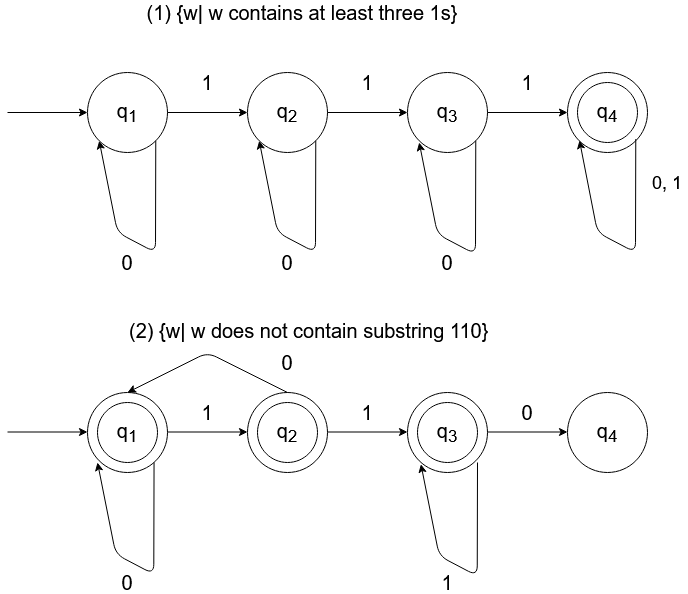
\includegraphics[scale=0.5]{Problem2Solution.png}
}

\newpage

\textbf{Problem \printnumbers .} A number is a prime if it cannot be a product of two numbers less than it. For examples, 2, 3, 5, 7, 11, 13 are prime numbers, but 6, 8, 10 are not. Prove by contradiction that there are infinite prime numbers.\\
\\
A twin number is a pair of prime numbers of difference 2. For examples, (3, 5), (11, 13), and (29, 31) are all twin numbers. Search internet about twin number conjecture. Provide its history and current research status.\\
Hint: Assume that there are only finite prime numbers \(p_{1}, p_{2}, \ldots, p_{k} \). Think about the number \(p_{1}*p_{2}* \ldots*p_{k}+1 \)

\textbf{\\Answer \printanswers . \\}
Assume that we have a finite number of prime numbers. If it is, then there is there are prime numbers \(p_{1}, p_{2}, \ldots, p_{k} \). Let's see if \(N = 1+p_{1}*p_{2}* \ldots*p_{k}\), because according to the lemma, N should have prime factorisation and \(N > p_{k} \).\\

If \(N\) is not prime, it means that we have \(p_{i}\) with \(1 \leq i \leq n \) that could be the divisor of both \(N\) and \(p_{1}*p_{2}* \ldots * p_{k}\). In this case, \(p_{i}\) is also the divisor of \(N - p_{1}*p_{2}* \ldots*p_{k}=1\). Because of \(p_{i} \geq 2 \), it is impossible, so we have the contradiction. As a result, we can conclude that there are an infinite number of primes.

\quad The history of twin number conjecture and the research status of the problem:
\begin{enumerate}
\item The question whether the number of twin primes is finite remains open.
\item In 1849, de Polignac stated that for every natural number \(k\), there are infinitely many primes \(p\) such that \(p + 2k\) is also prime. The case \(k=1\) is twin number conjecture.
\item The First Hardy–Littlewood conjecture says that for \(\pi_{2}(x)\) that denotes the number of primes \(p \leq x\) such that \(p + 2\) is also prime,

\[\pi_{2}(x) = 2C_{2} \frac{x}{{(\ln{x})}^{2}} \sim 2C_{2} \int_{2}^{x} \frac{dt}{{(\ln{t})}^{2}}\]
\\
where, 
\[C_{2} = \prod_{p \text{ is prime} \atop{p \geq 3}} \left (1-\frac{1}{{(p-1)}^{2}}  \right ) \approx 0.6601618158...\]
\item In 1915, Viggo Brun showed that the sum of reciprocals of the twin primes had the limit. Nowadays, it is determined that the limit doesn't exceed \[\frac{C'N}{(\log N)^{2}}\left ( 1+O\left ( \frac{\log \log N}{\log N} \right ) \right ), \text{where} \ C' = 8C_{2}\]

\item On April 17, 2013, Yitang Zhang announced a proof that there are infinite number of primes with the difference between the pair of primes not exceeding 70 millions. On April 14, 2014, by the collaborative effort of Polymath Project, the bound has been reduced to 246. Assuming to the Elliott–Halberstam conjecture and its generalized form, the bound has been reduced to 12 and 6, respectively.

\end{enumerate}


\vbox{
\textbf{Problem \printnumbers .}
\begin{enumerate}
\item Construct an NFA to accept \( L = \left \{a^{2n}b^{3m} \ : \ n \geq 1, m \geq 1\right \} \).
\item Construct an NFA to accept \( L = \left \{a^{n}b^{m} \ : \ n+m \ \text{is odd} \right \} \).
\end{enumerate}

\textbf{\\Answer \printanswers . In the picture, there are solutions of Problem 4:\\}

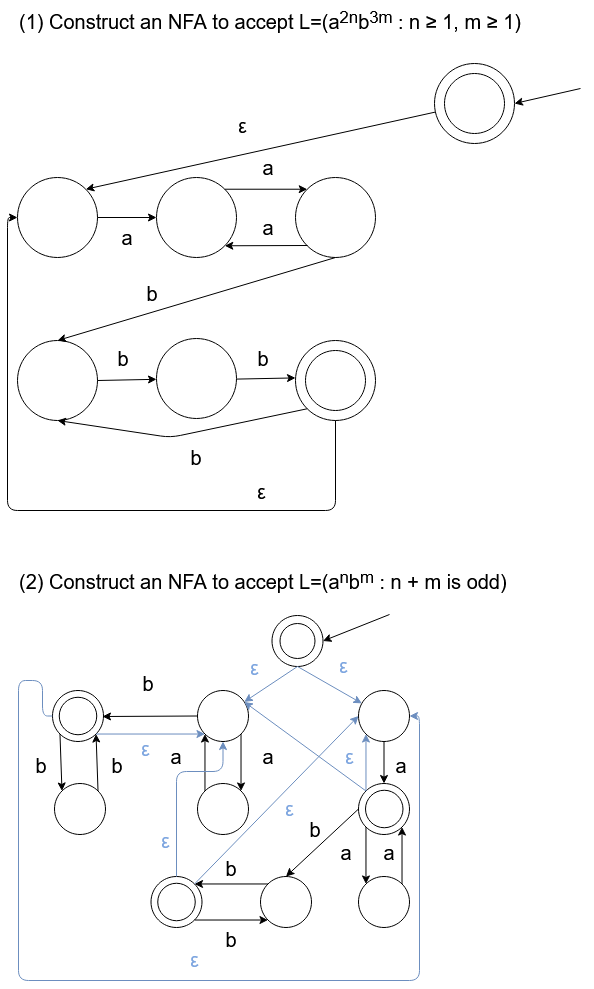
\includegraphics[scale=0.5]{Problem4Solution.png}
}

\newpage

\textbf{Problem \printnumbers .} Use the pumping lemma for the regular language to prove that the following languages are not regular.
\begin{enumerate}
\item \( A_{1} = \left \{0^{m}1^{n}2^{n} \ | \ m, n \geq 0 \right \} \).
\item \( A_{2} = \left \{0^{n}1^{n^{2}} \ | \ n \geq 0 \right \} \).
\end{enumerate}

\textbf{\\Answer \printanswers . \\}

\begin{enumerate}
\item Let's define \(|S| \geq |P| = m+2n\). To have  \(|xy| \leq |m+2n| \) we can choose \(x= 0^{m}\) and \( y = 1^{n}\) due to \(|xy| = m+n \leq |m+2n| \). So, \(|xyz| = 0^{m}1^{n}2^{n} \). Let's pump \(y\) to \(y^{2}\). After pumping, we have \( |S| = m+2n+n = |A_{1}|+n \). Due to the fact that \(n>0\), we don't have the regular language, because \(|xy^{2}z| = 0^{m}1^{2n}2^{n} \notin A_{1} \). In other words, we got 1's number higher than 2's, which is not possible. So, \(A_{1}\) is not regular.
\item Let's define \(|S| \geq |P| = |n+n^{2}|\), To have  \(|xy| \leq |n+n^{2}| \) we can choose \(x=0^{n}\) and define \(y = 1^{n}\) and \(z = 1^{n^{2}-n}\). Let's pump \(y\) to \(y^{2}\). Now, the \(|xy^{2}z| = 0^{n}1^{2n}1^{n^{2}-n} = 0^{n}1^{n}1^{n^{2}} \), which is not accepted by   \(A_{2}\). So, \(A_{2}\) is not regular due to the contradiction.
\end{enumerate}

\end{document}
